\documentclass{article}

\usepackage{amsmath}
\usepackage{amsthm}
\usepackage{mathtools}

\usepackage{tikz}
\usepackage{tkz-euclide}

\title{Algebrauppgift 6 - Basbyte i hexagon}
\author{Emma Bastås}
\date{November 6, 2022}

\begin{document}

\newcommand*\ee[0]{\overline{e}_{1}}
\newcommand*\eee[0]{\overline{e}_{2}}
\newcommand*\ff[0]{\overline{f}_{1}}
\newcommand*\fff[0]{\overline{f}_{2}}
\newcommand*\uu[0]{\overline{u}_{1}}
\newcommand*\uuu[0]{\overline{u}_{2}}

\maketitle


\noindent Betrakta en regelbunden sexhörning med hörn i punkterna $A$, $B$, $C$, $D$, $E$ och $F$ (i ordning motsols). Vektorerna $\ee = \overline{AB}$ och $\eee = \overline{AD}$ utgör en bas för planet liksom vektorerna $\ff = \overline{AC}$ och $\fff = \overline{AE}$. Det finns två uppgifter

\begin{enumerate}
        \item[a)] Vektorn $\overline{u}_{1}$ har kordinaterna $(5, -2)$ i basen $\ee, \eee$. Bestämm $\overline{u}_{2}$:s koordinater på avseende på basen $\ff, \fff$.
        \item[b)] Vektorn $\overline{u}_{2}$ har kordinaterna $(1, 6)$ i basen $\ff, \fff$. Bestämm $\overline{u}_{2}$:s koordinater på avseende på basen $\ee, \eee$.
\end{enumerate}

\noindent Vi börjar med att tolka detta geometriskt, en regelbunden hexagon består av sex liksidiga trianglar:

\begin{center}
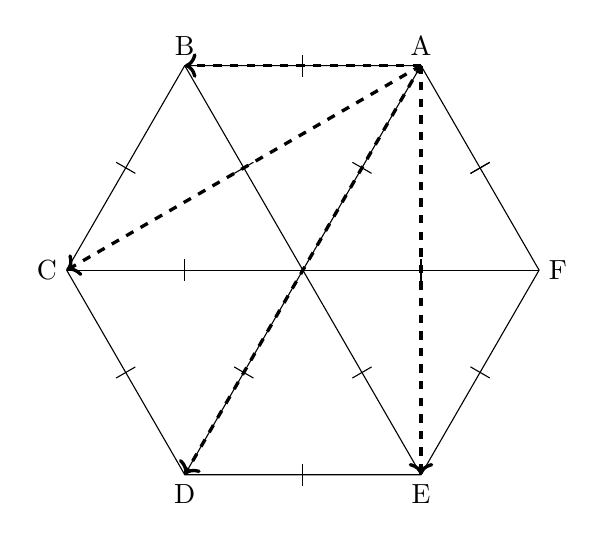
\begin{tikzpicture}[scale = 3]
  \coordinate[label=right:F] (F) at (0:1);
  \coordinate[label=A] (A) at (60:1);
  \coordinate[label=B] (B) at (120:1);
  \coordinate[label=left:C] (C) at (180:1);
  \coordinate[label=below:D] (D) at (240:1);
  \coordinate[label=below:E] (E) at (300:1);
  \coordinate (O) at (0,0);

  \draw (F)--(A)--(B)--(C)--(D)--(E)--cycle;
  \draw (C)--(O)--(F);
  \draw (A)--(O)--(D);
  \draw (B)--(O)--(E);

  \draw[->, very thick, dashed] (A)--(B) node[midway, above] {$\ee$};
  \draw[->, very thick, dashed] (A)--(C) node[midway, above] {$\ff$};
  \draw[->, very thick, dashed] (A)--(D) node[midway, above left] {$\eee$};
  \draw[->, very thick, dashed] (A)--(E) node[midway, above left] {$\fff$};

  \tkzMarkSegment (F,A);
  \tkzMarkSegment (F,E);
  \tkzMarkSegment (F,O);
  \tkzMarkSegment (F,A);
  \tkzMarkSegment (B,A);
  \tkzMarkSegment (B,C);
  \tkzMarkSegment (B,O);
  \tkzMarkSegment (D,C);
  \tkzMarkSegment (D,E);
  \tkzMarkSegment (D,O);
  \tkzMarkSegment (A,O);
  \tkzMarkSegment (C,O);
  \tkzMarkSegment (E,O);
\end{tikzpicture}
\end{center}

\noindent Med denna geometriska tolkning ser vi att:

\begin{equation}
  \begin{aligned}
    \ff &= \tfrac{1}{2}\eee + \ee \\
    \fff &= \eee - \ee\text{.}
  \end{aligned}
  \tag{$\star$}\label{*}
\end{equation}

%\begin{center}
%\begin{tikzpicture}[scale = 1.5]
%  \coordinate[label=A] (A) at (60:1);
%  \coordinate[label=B] (B) at (120:1);
%  \coordinate[label=left:C] (C) at (180:1);
%  \coordinate[label=below:D] (D) at (240:1);
%  \coordinate (O) at (0,0);
%
%  \draw[->] (A)--(B) node[midway, above] {$\ee$};
%  \draw[->] (A)--(C) node[midway, above] {$\ff$};
%  \draw[->] (B)--(C) node[midway, above left] {$\frac{1}{2}\eee$};
%  \draw[->] (A)--(D) node[midway, below right] {$\eee$};
%\end{tikzpicture}
%\quad\quad\quad\quad
%\begin{tikzpicture}[scale = 1.5]
%  \coordinate[label=A] (A) at (60:1);
%  \coordinate[label=B] (B) at (120:1);
%  \coordinate[label=below:D] (D) at (240:1);
%  \coordinate[label=below:E] (E) at (300:1);
%
%
%  \draw[->] (A)--(D) node[midway, above left] {$\eee$};
%  \draw[->] (A)--(E) node[midway, right] {$\fff$};
%  \draw[->] (A)--(B) node[midway, above] {$\ee$};
%  \draw[->] (D)--(E) node[midway, above] {$-\ee$};
%\end{tikzpicture}
%\end{center}

\newpage

\noindent Uppgift b)
\\
\\
Vi ställer upp $\uuu$ som en linjärkombination av $\ff$ och $\fff$:

\begin{gather*}
  \uuu = \ff + 6\fff
\end{gather*}

\noindent och skriver om detta som en linjärkombination av $\ee$ och $\eee$ med hjälp av (\ref{*}):

\begin{align*}
  \uuu &= (\tfrac{1}{2}\eee + \ee) + 6(\eee - \ee)\\[2pt]
  & = \tfrac{13}{2}\eee - 5\ee\text{.}
\end{align*}
\\
\\
Uppgift a)
\\
\\
Vi skriver om ekvationerna i (\ref{*}) så att $\ee$ och $\eee$ är linjärkombnationer av $\ff$ och $\fff$:

\begin{gather}
  \text{(\ref{*})} \quad \iff \quad
  \begin{aligned}
    \ee &= \tfrac{2}{3}\ff - \tfrac{1}{3}\fff\\
    \eee &= \tfrac{2}{3}(\ff + \fff)
  \end{aligned}\text{.} \tag{$\star\star$}\label{**}
\end{gather}
\\
Vi ställer nu upp $\uu$ som en linjärkombination av $\ee$ och $\eee$:

\begin{gather*}
  \uu = 5\ee - 2\eee
\end{gather*}
\\
och skriver om detta som en linjärkombination av $\ff$ och $\fff$ med hjälp av (\ref{**}):

\begin{align*}
  \uu &= 5\ee - 2\eee\\
  & = 5(\tfrac{2}{3}\ff - \tfrac{1}{3}\fff) - 2\tfrac{2}{3}(\ff + \fff)\\
  &= 2\ff - 3\fff\text{.}
\end{align*}
\end{document}
